\KNEADSECTIONNEWPAGE
\section{Capabilities}
\label{lab:sec_Capabilities}
\RequirementNumberAM{section}{3.3}
% \DIDINFO{SPS/SSS-3.3.0 :: This section shall be divided into subparagraphs to itemize the requirements associated with each capability of the system. 
A ``capability'' is defined as a group of related requirements. 
The word ``capability'' may be replaced with ``function'', ``subject'', ``object'', or other term useful for presenting the requirements.}



%\newcommand{\ThisCapability}{Capabilities UNDEFINED}

This section defines the capability areas for the \ThisSys.
The segment design is structured to meet the requirements as specified in the \SPS \citeExProjSPS and \SSS \citeExProjSSS artifacts.
Each area provides a subset of the overall capabilities for the \ThisSys segments.
These segments are shown in Figure~\ref{fig:DFD-0}, are summarized below, and are more fully specified in the following subsections.
\begin{figure}[htbp]
	\centering
		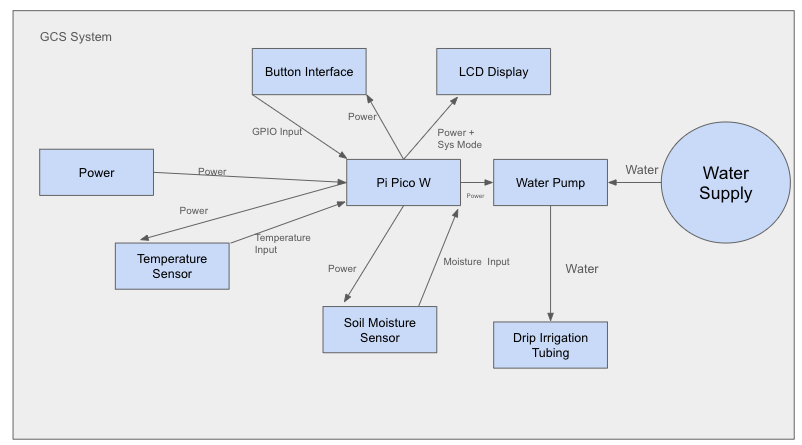
\includegraphics[width=6.5in]{/Users/zsteinberg/UMD/ENPM818I/LatexInputs/ExampleArtifactFolders/zProjectWideData/images/SYS-DFD-0.png}
	\caption[System Top-Level Diagram]{System Top-Level Diagram (DFD-0)}
	\label{fig:DFD-0}
\end{figure}
 
The capability requirements for these segments are described in more detail in the following sections:
\begin{description}
	\item[Operator Processing] handles the \HMI interface to the operator and provides overall control and configuration to the \ThisSys, \S~\ref{loc:Capability_Operator}.
	\item[Network Processing] handles the network interface, \S~\ref{loc:Capability_Network}.
	\item[Power Processing] handles the power input and conversions as necessary, \S~\ref{loc:Capability_Power}.
	\item[Control Processing] handles all major capability control, \S~\ref{loc:Capability_Control}.
\end{description}

%%%%%%%%%%%%%%%%%%%%%%%%%%%%%%%%%%%%%%%%%%%%%%%%%%%%%%%%%%%%%%%%%%%%%%%%%%%%%%%%
%%%%%%%%%%%%%%%%%%%%%%%%%%%%%%%%%%%%%%%%%%%%%%%%%%%%%%%%%%%%%%%%%%%%%%%%%%%%%%%
%\KNEADSUBSECTIONNEWPAGE
\newpage
\subsection{Operator Processing}
\label{loc:Capability_Operator}
\RequirementNumberAM{subsection}{3.3.1}

The operator requirements for \ThisSystem are listed below.

%%% \ONERQMTV[9] is macro for consistently formatted requirements
\ONERQMTVKPP
% #1 is requirement Number
{\RqtNumberBase.1}
% #2 is Title
{Garden Drip Irrigation}
% #3 is requirement label (expected to be of form rqt:XXX)
{rqt:Operator Outputs}
% #4 is Text of the specification
{All \ThisSys variants shall be capable of proper garden drip irrigation until environmental thresholds are met or a set time duration has passed. The drip irrigation system will be made up of Rain Bird Drip Irrigation Tubing.}
% #5 is Status (S in {(T), (O), (I), (D)} listed by phase as \item [] S)
{
	\item [All Phases] Threshold
}
% #6 is Acceptance
{This requirement shall be verified by demonstration.}
% #7 is Traceability
{
	\item [N/A] This requirement is a base requirement.
}
% #8 is Notes; listed as enumeration \item ...
{
  \item The irrigation system will be capable of watering a garden of a set size.
  \item \href{https://www.homedepot.com/p/Rain-Bird-1-2-in-0-71-in-O-D-x-100-ft-Distribution-Tubing-for-Drip-Irrigation-T70-100S/204751445}{Rain Bird Tubing}
}
% #9 is changebar version
{P1}
%%%%% end \ONERQMTV[9] macro

%%% \ONERQMTV[9] is macro for consistently formatted requirements
\ONERQMTVKPP
% #1 is requirement Number
{\RqtNumberBase.2}
% #2 is Title
{Water Pump}
% #3 is requirement label (expected to be of form rqt:XXX)
{rqt:Operator Outputs}
% #4 is Text of the specification
{All \ThisSys variants shall be capable activating and deactivating a US Solar Pump B3A 5V PWM Circulating water pump. The water pump will send water to a drip irrigation system and will be capable of running for 24-hours.}
% #5 is Status (S in {(T), (O), (I), (D)} listed by phase as \item [] S)
{
	\item [All Phases] Threshold
}
% #6 is Acceptance
{This requirement shall be verified by demonstration.}
% #7 is Traceability
{
	\item [N/A] This requirement is a base requirement.
}
% #8 is Notes; listed as enumeration \item ...
{
  \item The water pump will control water flow to an irrigation system.
  \item \href{https://www.ussolarpumps.com/catalog/5v-pwm-wired-pumps/b3a-5v-pwm-circulating-pump/}{US Solar Pump B3A 5V PWM Circulating Water Pump Product Page}
}
% #9 is changebar version
{P1}
%%%%% end \ONERQMTV[9] macro

%%% \ONERQMTV[9] is macro for consistently formatted requirements
\ONERQMTVKPP
% #1 is requirement Number
{\RqtNumberBase.3}
% #2 is Title
{Temperature Measurements}
% #3 is requirement label (expected to be of form rqt:XXX)
{rqt:Operator Inputs}
% #4 is Text of the specification
{All \ThisSys variants shall be capable of measuring temperature through the BME280 Temperature Sensor.}
% #5 is Status (S in {(T), (O), (I), (D)} listed by phase as \item [] S)
{
	\item [All Phases] Threshold
}
% #6 is Acceptance
{This requirement shall be verified by demonstration.}
% #7 is Traceability
{
	\item [N/A] This requirement is a base requirement.
}
% #8 is Notes; listed as enumeration \item ...
{
  \item Temperature will be measured via the \ThisSys temperature sensor.
}
% #9 is changebar version
{P1}
%%%%% end \ONERQMTV[9] macro

%%% \ONERQMTV[9] is macro for consistently formatted requirements
\ONERQMTVKPP
% #1 is requirement Number
{\RqtNumberBase.4}
% #2 is Title
{Soil Moisture Measurements}
% #3 is requirement label (expected to be of form rqt:XXX)
{rqt:Operator Inputs}
% #4 is Text of the specification
{All \ThisSys variants shall be capable of measuring soil moisture levels through the I2C Capacitive Moisture Sensor.}
% #5 is Status (S in {(T), (O), (I), (D)} listed by phase as \item [] S)
{
	\item [All Phases] Threshold
}
% #6 is Acceptance
{This requirement shall be verified by demonstration.}
% #7 is Traceability
{
	\item [N/A] This requirement is a base requirement.
}
% #8 is Notes; listed as enumeration \item ...
{
  \item Soil moisture will be measured via the \ThisSys soil moisture sensor.
  \item \href{https://learn.adafruit.com/adafruit-stemma-soil-sensor-i2c-capacitive-moisture-sensor}{Datasheet}
}
% #9 is changebar version
{P1}
%%%%% end \ONERQMTV[9] macro


%%% \ONERQMTV[9] is macro for consistently formatted requirements
\ONERQMTVKPP
% #1 is requirement Number
{\RqtNumberBase.5}
% #2 is Title
{\ThisSys Mode Toggling}
% #3 is requirement label (expected to be of form rqt:XXX)
{rqt:Operator Inputs}
% #4 is Text of the specification
{All \ThisSys variants shall be capable of toggling through set modes via a button interface connected to GPIO Pins.}
% #5 is Status (S in {(T), (O), (I), (D)} listed by phase as \item [] S)
{
	\item [All Phases] Threshold
}
% #6 is Acceptance
{This requirement shall be verified by demonstration.}
% #7 is Traceability
{
	\item [N/A] This requirement is a base requirement.
}
% #8 is Notes; listed as enumeration \item ...
{
  \item Button interface will switch the active \GCS mode.
  \item \item \href{https://projects.raspberrypi.org/en/projects/introduction-to-the-pico/10}{Raspberry Pi Pico Button Guide}
}
% #9 is changebar version
{P1}
%%%%% end \ONERQMTV[9] macro

%%% \ONERQMTV[9] is macro for consistently formatted requirements
\ONERQMTVKPP
% #1 is requirement Number
{\RqtNumberBase.6}
% #2 is Title
{\ThisSys Mode Display}
% #3 is requirement label (expected to be of form rqt:XXX)
{rqt:Operator Inputs}
% #4 is Text of the specification
{All \ThisSys variants shall be capable of displaying it's active mode via an Adafruit Standard HD44780 LCD Display.}
% #5 is Status (S in {(T), (O), (I), (D)} listed by phase as \item [] S)
{
	\item [All Phases] Threshold
}
% #6 is Acceptance
{This requirement shall be verified by demonstration.}
% #7 is Traceability
{
	\item [N/A] This requirement is a base requirement.
}
% #8 is Notes; listed as enumeration \item ...
{
  \item An LCD display will show the active \GCS mode.
  \item \href{https://cdn-shop.adafruit.com/datasheets/HD44780.pdf}{Datasheet}
}
% #9 is changebar version
{P1}
%%%%% end \ONERQMTV[9] macro


%%%%%%%%%%%%%%%%%%%%%%%%%%%%%%%%%%%%%%%%%%%%%%%%%%%%%%%%%%%%%%%%%%%%%%%%%%%%%%%
%%%%%%%%%%%%%%%%%%%%%%%%%%%%%%%%%%%%%%%%%%%%%%%%%%%%%%%%%%%%%%%%%%%%%%%%%%%%%%%
%\KNEADSUBSECTIONNEWPAGE
\newpage
\subsection{Network Processing}
\label{loc:Capability_Network}
\RequirementNumberAM{subsection}{3.3.2}

The network requirements for \ThisSystem are listed below.


%%% \ONERQMTV[9] is macro for consistently formatted requirements
\ONERQMTVKPP
% #1 is requirement Number
{\RqtNumberBase.1}
% #2 is Title
{Network Types}
% #3 is requirement label (expected to be of form rqt:XXX)
{rqt:NetworkTypes}
% #4 is Text of the specification
{All \ThisSys variants shall be capable of \TBD network types.}
% #5 is Status (S in {(T), (O), (I), (D)} listed by phase as \item [] S)
{
	\item [Phase 1] Threshold
}
% #6 is Acceptance
{This requirement shall be verified by demonstration.}
% #7 is Traceability
{
	\item [N/A] This requirement is a base requirement.
}
% #8 is Notes; listed as enumeration \item ...
{
  \item Add as many of these as necessary.  Split into files/folders, e.g., NetworkTypes.tex, NetworkInputs.tex, and NetworkOutputs.tex, etc. as needed. Just use the RequirementNumberAM and RqtNumberBase commands to keep numbers correct if subsubsections are added.
}
% #9 is changebar version
{P1}
%%%%% end \ONERQMTV[9] macro


%%% \ONERQMTV[9] is macro for consistently formatted requirements
\ONERQMTVKPP
% #1 is requirement Number
{\RqtNumberBase.2}
% #2 is Title
{Network Inputs}
% #3 is requirement label (expected to be of form rqt:XXX)
{rqt:NetworkInputs}
% #4 is Text of the specification
{All \ThisSys variants shall be capable of \TBD network inputs.}
% #5 is Status (S in {(T), (O), (I), (D)} listed by phase as \item [] S)
{
	\item [Phase 1] Threshold
}
% #6 is Acceptance
{This requirement shall be verified by demonstration.}
% #7 is Traceability
{
	\item [N/A] This requirement is a base requirement.
}
% #8 is Notes; listed as enumeration \item ...
{
  \item Add as many of these as necessary.  Split into files/folders, e.g., NetworkTypes.tex, NetworkInputs.tex, and NetworkOutputs.tex, etc. as needed. Just use the RequirementNumberAM and RqtNumberBase commands to keep numbers correct if subsubsections are added.
}
% #9 is changebar version
{P1}
%%%%% end \ONERQMTV[9] macro

%%% \ONERQMTV[9] is macro for consistently formatted requirements
\ONERQMTVKPP
% #1 is requirement Number
{\RqtNumberBase.3}
% #2 is Title
{Network Outputs}
% #3 is requirement label (expected to be of form rqt:XXX)
{rqt:NetworkOutputs}
% #4 is Text of the specification
{All \ThisSys variants shall be capable of \TBD network outputs.}
% #5 is Status (S in {(T), (O), (I), (D)} listed by phase as \item [] S)
{
	\item [Phase 1] Threshold
}
% #6 is Acceptance
{This requirement shall be verified by demonstration.}
% #7 is Traceability
{
	\item [N/A] This requirement is a base requirement.
}
% #8 is Notes; listed as enumeration \item ...
{
  \item Add as many of these as necessary.  Split into files/folders, e.g., NetworkTypes.tex, NetworkInputs.tex, and NetworkOutputs.tex, etc. as needed. Just use the RequirementNumberAM and RqtNumberBase commands to keep numbers correct if subsubsections are added.
}
% #9 is changebar version
{P1}
%%%%% end \ONERQMTV[9] macro



%%%%%%%%%%%%%%%%%%%%%%%%%%%%%%%%%%%%%%%%%%%%%%%%%%%%%%%%%%%%%%%%%%%%%%%%%%%%%%%
%%%%%%%%%%%%%%%%%%%%%%%%%%%%%%%%%%%%%%%%%%%%%%%%%%%%%%%%%%%%%%%%%%%%%%%%%%%%%%%
%\KNEADSUBSECTIONNEWPAGE
\newpage
\subsection{Power Processing}
\label{loc:Capability_Power}
\RequirementNumberAM{subsection}{3.3.3}

%%% \ONERQMTV[9] is macro for consistently formatted requirements
\ONERQMTVKPP
% #1 is requirement Number
{\RqtNumberBase.2}
% #2 is Title
{US Solar Pump B3A 5V PWM Circulating Pump Power}
% #3 is requirement label (expected to be of form rqt:XXX)
{rqt:Power}
% #4 is Text of the specification
{All \ThisSys variants shall be capable of routing and supplying 5V of power to the US Solar Pump B3A 5V PWM Circulating Pump.}
% #5 is Status (S in {(T), (O), (I), (D)} listed by phase as \item [] S)
{
	\item [All Phases] Threshold
}
% #6 is Acceptance
{This requirement shall be verified by demonstration.}
% #7 is Traceability
{
	\item [N/A] This requirement is a base requirement.
}
% #8 is Notes; listed as enumeration \item ...
{
	\item \href{https://www.ussolarpumps.com/catalog/5v-pwm-wired-pumps/b3a-5v-pwm-circulating-pump/}{Product Page}
}
% #9 is changebar version
{P1}
%%%%% end \ONERQMTV[9] macro

%%% \ONERQMTV[9] is macro for consistently formatted requirements
\ONERQMTVKPP
% #1 is requirement Number
{\RqtNumberBase.3}
% #2 is Title
{BME280 Temperature Sensor Power}
% #3 is requirement label (expected to be of form rqt:XXX)
{rqt:Power}
% #4 is Text of the specification
{All \ThisSys variants shall be capable of routing and supplying between 1.2V-3.6V of power to the BME280 Temperature Sensor.}
% #5 is Status (S in {(T), (O), (I), (D)} listed by phase as \item [] S)
{
	\item [All Phases] Threshold
}
% #6 is Acceptance
{This requirement shall be verified by demonstration.}
% #7 is Traceability
{
	\item [N/A] This requirement is a base requirement.
}
% #8 is Notes; listed as enumeration \item ...
{
    \item \href{https://cdn-learn.adafruit.com/assets/assets/000/115/588/original/bst-bme280-ds002.pdf?1664822559}{Datasheet}
  	\item \href{https://github.com/adafruit/Adafruit_BME280_Library}{BME280 Driver}
}
% #9 is changebar version
{P1}
%%%%% end \ONERQMTV[9] macro

%%% \ONERQMTV[9] is macro for consistently formatted requirements
\ONERQMTVKPP
% #1 is requirement Number
{\RqtNumberBase.4}
% #2 is Title
{I2C Capacitive Moisture Sensor Power Requirements}
% #3 is requirement label (expected to be of form rqt:XXX)
{rqt:Power}
% #4 is Text of the specification
{All \ThisSys variants shall be capable of routing and supplying between 3V-5V of power to the BME280 Temperature Sensor.}
% #5 is Status (S in {(T), (O), (I), (D)} listed by phase as \item [] S)
{
	\item [All Phases] Threshold
}
% #6 is Acceptance
{This requirement shall be verified by demonstration.}
% #7 is Traceability
{
	\item [N/A] This requirement is a base requirement.
}
% #8 is Notes; listed as enumeration \item ...
{
	\item \href{https://learn.adafruit.com/adafruit-stemma-soil-sensor-i2c-capacitive-moisture-sensor}{Datasheet}
}
% #9 is changebar version
{P1}
%%%%% end \ONERQMTV[9] macro

%%% \ONERQMTV[9] is macro for consistently formatted requirements
\ONERQMTVKPP
% #1 is requirement Number
{\RqtNumberBase.5}
% #2 is Title
{Adafruit Standard HD44780 LCD Power Requirements}
% #3 is requirement label (expected to be of form rqt:XXX)
{rqt:Power}
% #4 is Text of the specification
{All \ThisSys variants shall be capable of routing and supplying between 2.7V - 5V of power to the Adafruit Standard HD44780 LCD.}
% #5 is Status (S in {(T), (O), (I), (D)} listed by phase as \item [] S)
{
	\item [All Phases] Threshold
}
% #6 is Acceptance
{This requirement shall be verified by demonstration.}
% #7 is Traceability
{
	\item [N/A] This requirement is a base requirement.
}
% #8 is Notes; listed as enumeration \item ...
{
	\item \href{https://cdn-shop.adafruit.com/datasheets/HD44780.pdf}{Datasheet}
}
% #9 is changebar version
{P1}
%%%%% end \ONERQMTV[9] macro





%%%%%%%%%%%%%%%%%%%%%%%%%%%%%%%%%%%%%%%%%%%%%%%%%%%%%%%%%%%%%%%%%%%%%%%%%%%%%%%%
%%%%%%%%%%%%%%%%%%%%%%%%%%%%%%%%%%%%%%%%%%%%%%%%%%%%%%%%%%%%%%%%%%%%%%%%%%%%%%%
%\KNEADSUBSECTIONNEWPAGE
\newpage
\subsection{Control Processing}
\label{loc:Capability_Control}
\RequirementNumberAM{subsection}{3.3.4}

The control requirements for \ThisSystem are listed below.

%%% \ONERQMTV[9] is macro for consistently formatted requirements
\ONERQMTVKPP
% #1 is requirement Number
{\RqtNumberBase.1}
% #2 is Title
{Control One}
% #3 is requirement label (expected to be of form rqt:XXX)
{rqt:ControlOne}
% #4 is Text of the specification
{All \ThisSys variants shall be capable of \TBD control one.}
% #5 is Status (S in {(T), (O), (I), (D)} listed by phase as \item [] S)
{
	\item [Phase 1] Threshold
}
% #6 is Acceptance
{This requirement shall be verified by demonstration.}
% #7 is Traceability
{
	\item [N/A] This requirement is a base requirement.
}
% #8 is Notes; listed as enumeration \item ...
{
  \item Add as many of these as necessary.  Split into files/folders as needed for areas of control capabilities. Just use the RequirementNumberAM and RqtNumberBase commands to keep numbers correct if subsubsections are added.
}
% #9 is changebar version
{P1}
%%%%% end \ONERQMTV[9] macro

%%% \ONERQMTV[9] is macro for consistently formatted requirements
\ONERQMTVKPP
% #1 is requirement Number
{\RqtNumberBase.2}
% #2 is Title
{Control Two}
% #3 is requirement label (expected to be of form rqt:XXX)
{rqt:ControlTwo}
% #4 is Text of the specification
{All \ThisSys variants shall be capable of \TBD control two.}
% #5 is Status (S in {(T), (O), (I), (D)} listed by phase as \item [] S)
{
	\item [Phase 1] Threshold
}
% #6 is Acceptance
{This requirement shall be verified by demonstration.}
% #7 is Traceability
{
	\item [N/A] This requirement is a base requirement.
}
% #8 is Notes; listed as enumeration \item ...
{
  \item Add as many of these as necessary.  Split into files/folders as needed for areas of control capabilities. Just use the RequirementNumberAM and RqtNumberBase commands to keep numbers correct if subsubsections are added.
}
% #9 is changebar version
{P1}
%%%%% end \ONERQMTV[9] macro